% Options for packages loaded elsewhere
\PassOptionsToPackage{unicode}{hyperref}
\PassOptionsToPackage{hyphens}{url}
\documentclass[
]{article}
\usepackage{xcolor}
\usepackage{amsmath,amssymb}
\setcounter{secnumdepth}{-\maxdimen} % remove section numbering
\usepackage{iftex}
\ifPDFTeX
  \usepackage[T1]{fontenc}
  \usepackage[utf8]{inputenc}
  \usepackage{textcomp} % provide euro and other symbols
\else % if luatex or xetex
  \usepackage{unicode-math} % this also loads fontspec
  \defaultfontfeatures{Scale=MatchLowercase}
  \defaultfontfeatures[\rmfamily]{Ligatures=TeX,Scale=1}
\fi
\usepackage{lmodern}
\ifPDFTeX\else
  % xetex/luatex font selection
\fi
% Use upquote if available, for straight quotes in verbatim environments
\IfFileExists{upquote.sty}{\usepackage{upquote}}{}
\IfFileExists{microtype.sty}{% use microtype if available
  \usepackage[]{microtype}
  \UseMicrotypeSet[protrusion]{basicmath} % disable protrusion for tt fonts
}{}
\makeatletter
\@ifundefined{KOMAClassName}{% if non-KOMA class
  \IfFileExists{parskip.sty}{%
    \usepackage{parskip}
  }{% else
    \setlength{\parindent}{0pt}
    \setlength{\parskip}{6pt plus 2pt minus 1pt}}
}{% if KOMA class
  \KOMAoptions{parskip=half}}
\makeatother
\usepackage{longtable,booktabs,array}
\usepackage{calc} % for calculating minipage widths
% Correct order of tables after \paragraph or \subparagraph
\usepackage{etoolbox}
\makeatletter
\patchcmd\longtable{\par}{\if@noskipsec\mbox{}\fi\par}{}{}
\makeatother
% Allow footnotes in longtable head/foot
\IfFileExists{footnotehyper.sty}{\usepackage{footnotehyper}}{\usepackage{footnote}}
\makesavenoteenv{longtable}
\usepackage{graphicx}
\makeatletter
\newsavebox\pandoc@box
\newcommand*\pandocbounded[1]{% scales image to fit in text height/width
  \sbox\pandoc@box{#1}%
  \Gscale@div\@tempa{\textheight}{\dimexpr\ht\pandoc@box+\dp\pandoc@box\relax}%
  \Gscale@div\@tempb{\linewidth}{\wd\pandoc@box}%
  \ifdim\@tempb\p@<\@tempa\p@\let\@tempa\@tempb\fi% select the smaller of both
  \ifdim\@tempa\p@<\p@\scalebox{\@tempa}{\usebox\pandoc@box}%
  \else\usebox{\pandoc@box}%
  \fi%
}
% Set default figure placement to htbp
\def\fps@figure{htbp}
\makeatother
\setlength{\emergencystretch}{3em} % prevent overfull lines
\providecommand{\tightlist}{%
  \setlength{\itemsep}{0pt}\setlength{\parskip}{0pt}}
\usepackage{bookmark}
\IfFileExists{xurl.sty}{\usepackage{xurl}}{} % add URL line breaks if available
\urlstyle{same}
\hypersetup{
  pdftitle={NeuroBeat: Validation-Locked and Energy-Accounted Spiking Networks for Inter-Patient Ventricular Ectopic Beat Detection},
  pdfauthor={Valerio Merlini},
  hidelinks,
  pdfcreator={LaTeX via pandoc}}

\title{NeuroBeat: Validation-Locked and Energy-Accounted Spiking
Networks for Inter-Patient Ventricular Ectopic Beat Detection}
\author{Valerio Merlini}
\date{July 2026}

\begin{document}
\maketitle

Independent researcher\\
Contact: valerio@covenance.ai\\
Code, weights, and live dashboard: github.com/Talch87/neuro-beat and
talch87.github.io/neuro-beat

\subsection{Abstract}\label{abstract}

\textbf{Problem.} Spiking neural networks (SNNs) are attractive for
always-on cardiac monitoring because event-driven computation maps onto
low-power neuromorphic hardware. Yet much of the SNN-ECG literature
reports accuracy under protocols that inflate it (intra-patient splits,
test-set-selected thresholds) and rarely reports the per-inference
compute that motivates the approach.

\textbf{Approach.} We present NeuroBeat, a deliberately simple
leaky-integrate-and-fire network for ventricular ectopic beat (VEB)
detection, evaluated under a conservative protocol: a patient-disjoint
inter-patient split (MIT-BIH DS1 to DS2), an operating point fit only on
a DS1 validation holdout and then frozen for all test data, an explicit
per-beat synaptic-operation (SynOps) budget, and frozen cross-database
testing on two external databases.

\textbf{Result.} No single operating point reaches both high sensitivity
and high precision (VEB sensitivity 0.894 at PPV 0.490, or 0.857 at
0.679), consistent with calibration variance under a small holdout. A
gated-ensemble cascade, in which a sparse high-recall screener gates a
three-seed confirmer on the roughly 27\% of beats it flags, reaches VEB
sensitivity 0.923 at PPV 0.616 on DS2 within 23,385 SynOps/beat and
holds sensitivity at or above 0.90 across DS2, SVDB, and INCART under
one frozen operating point. A patient-level bootstrap gives wide
intervals (sensitivity 0.850 to 0.976, PPV 0.355 to 0.814), the honest
uncertainty for 22 test patients; with a standard R-peak detector
instead of annotations, end-to-end detection falls modestly to 0.884 /
0.593.

\textbf{Limitations.} SynOps is a compute proxy, not measured energy,
and stronger non-spiking baselines match or beat the cascade on
accuracy, so the spiking model's case rests on per-beat operation count
rather than accuracy. Single-lead supraventricular (SVEB) detection is
an unresolved negative result. The contribution is a validation-locked,
energy-accounted evaluation pattern and a cascade that improves the
sensitivity/PPV/energy tradeoff, positioning the method as a candidate
low-power VEB screening component, not a diagnostic system.

\subsection{1. Introduction}\label{introduction}

Long-term ambulatory ECG is increasingly recorded by wearable and patch
devices that must operate for days on a small battery. Ventricular
ectopic beats are clinically meaningful: their frequency and patterning
(for example couplets and non-sustained ventricular runs) are used in
risk stratification, and reliable beat labelling underpins Holter
reporting. A detector intended for continuous, on-device operation
therefore has two coupled requirements: it must be sensitive, because
missed ventricular beats are the costly error, and it must be
inexpensive per beat, because energy determines battery life and thermal
envelope.

Spiking networks are a candidate for this regime. They compute with
sparse binary events, and on neuromorphic substrates the dominant cost
is the number of synaptic operations actually triggered by spikes rather
than a fixed clocked cost per layer. This has motivated a body of
SNN-ECG work. Our reading of that literature, consistent with a recent
systematic review {[}Silva2025{]}, is that two recurring issues limit
how far its accuracy numbers can be trusted for deployment.

First, evaluation is frequently optimistic. Under an intra-patient
split, beats from the same patient appear in both training and test
sets, so the model can exploit patient-specific morphology that a device
deployed on a new patient never observes; reported accuracy then
overstates real inter-patient performance. Separately, selecting the
decision threshold (or per-class bias) on the test set leaks label
information that is unavailable at deployment time, again inflating the
headline metric. Neither practice is exotic; both are common enough that
cross-study comparison is unreliable {[}Silva2025{]}.

Second, energy is usually not accounted for. The stated reason to use an
SNN is efficiency, yet many reports give only accuracy or parameter
counts, with no per-inference operation budget against which efficiency
could be judged.

The contribution of this paper is therefore not a novel architecture.
The network is intentionally small and conventional. The contribution is
evaluation discipline and an energy-accounted deployment framing: an
operating point that is locked on validation data and never touched on
test data, an explicit SynOps budget applied to every configuration,
frozen cross-database testing, and a gated cascade that improves the
sensitivity/PPV/energy tradeoff within that budget. We also report,
rather than hide, a clear negative result for supraventricular beats on
a single lead.

\textbf{Contributions.}

\begin{enumerate}
\def\labelenumi{\arabic{enumi}.}
\tightlist
\item
  \textbf{A validation-locked inter-patient protocol.} We adopt the de
  Chazal DS1/DS2 patient-disjoint split {[}deChazal2004{]}, hold out
  three DS1 records as a patient-disjoint validation set, fit the
  operating point only on that holdout, and freeze it for DS2 and all
  external data. No reported test number participates in selecting the
  operating point on the split it is reported on (Section 6).
\item
  \textbf{An explicit per-beat SynOps budget.} We define a per-beat
  synaptic-operation count (Section 5.4), report it for every
  configuration, and hold each to a fixed 25,000 SynOps/beat budget.
\item
  \textbf{Frozen cross-database validation.} The single frozen operating
  point is applied unchanged to two databases the model never trained on
  (SVDB, INCART), quantifying transfer under distribution shift.
\item
  \textbf{A gated-ensemble cascade within budget.} A sparse screener on
  every beat gates a small ensemble confirmer on flagged beats, reaching
  VEB sensitivity 0.923 at PPV 0.616 within 23,385 SynOps/beat, which no
  single-stage model in our sweep achieves.
\item
  \textbf{A negative result for single-lead SVEB.} Under the same
  protocol, single-lead supraventricular detection does not reach usable
  precision, and we document why and how it fails rather than tuning it
  to a misleading number.
\end{enumerate}

\subsection{2. Related Work}\label{related-work}

\textbf{(a) ECG arrhythmia classification and inter-patient evaluation.}
The ANSI/AAMI EC57 standard {[}AAMI-EC57{]} defines the five heartbeat
classes and the sensitivity/PPV reporting convention used throughout
this literature. de Chazal et al.~{[}deChazal2004{]} introduced the
patient-disjoint DS1/DS2 partition of the 44 non-paced MIT-BIH records
(about 50,000 beats per set) that has become the reference inter-patient
benchmark. Many subsequent methods report higher raw accuracy than we
do, but a substantial share do so under intra-patient splits or with
test-set-selected thresholds; the systematic review of Silva et al.
{[}Silva2025{]} documents that few studies simultaneously satisfy
inter-patient partitioning, AAMI compliance, and embedded feasibility.
We do not claim to beat the strongest reported numbers on raw accuracy;
we claim comparability under a stricter, leakage-controlled protocol
with an energy budget.

\textbf{(b) Low-power and embedded ECG inference.} A parallel line of
work targets resource-constrained deployment through quantized and
compact convolutional or temporal-convolutional models, pruning, and
microcontroller implementations. These approaches report MACs, memory
footprint, or measured microcontroller energy. They are the natural
non-spiking comparison point for efficiency claims; we include
convolutional, recurrent, temporal-convolutional, residual-CNN,
gradient-boosted-tree, and SVM baselines, plus a weight-only int8 CNN,
under the identical protocol (Section 7.8).

\textbf{(c) Spiking and neuromorphic ECG.} SNN-ECG methods report
competitive MIT-BIH accuracy using delta-modulation encoding of the ECG
and its derivatives {[}SNN-ECG-BSPC2021{]}, spike-driven processors for
wearable ECG {[}Chu2022{]}, hardware/software co-design
{[}SparrowSNN2024{]}, and axonal-delay models {[}AxonalDelays2025{]}.
Our count-pooled delta encoding over signal orders is in this family. We
differ in evaluation rather than in mechanism: we report validation-
locked inter-patient results with an explicit SynOps budget, frozen
cross-database transfer, and a documented single-lead SVEB failure.

\textbf{(d) Cascaded and gated inference.} Two-stage screener/confirmer
and energy-gated designs are established elsewhere for trading average
compute against accuracy. We use the pattern narrowly: to make an
ensemble-grade confirmer affordable on average by invoking it only on
candidates a cheap screener flags.

\textbf{(e) Evaluation hygiene and reproducibility.} Our protocol
choices follow the recommendations surveyed in {[}Silva2025{]}. We
additionally release code, frozen weights, per-seed logs, and a public
results page so that every reported number is regenerable.

\subsection{3. Data}\label{data}

\textbf{MIT-BIH Arrhythmia Database (primary).} 48 two-lead ambulatory
records sampled at 360 Hz. Annotated beats are mapped to the five AAMI
classes: N (normal), S (supraventricular ectopic, SVEB), V (ventricular
ectopic, VEB), F (fusion of normal and ventricular), and Q
(unknown/paced). We use the de Chazal patient-disjoint split
{[}deChazal2004{]}: DS1 for training and DS2 for test, with no patient
in both. From DS1 we hold out records 201, 207, and 223 as a
patient-disjoint validation set used only for operating-point selection.
Beat counts are given in Table 1.

\textbf{External databases (test-only).} The MIT-BIH Supraventricular
Arrhythmia Database (SVDB, 128 Hz) {[}SVDB{]} and the St.~Petersburg
INCART 12-lead Arrhythmia Database (INCART, 257 Hz) {[}INCART{]}. These
are used exclusively for frozen cross-database testing; no external beat
enters training or operating-point selection for the VEB models.

\textbf{Preprocessing and resampling.} External signals are resampled to
360 Hz with polyphase resampling (\texttt{scipy.signal.resample\_poly},
applied to the ratio reduced by its greatest common divisor), and
annotation sample indices are rescaled by the same factor. Lead
selection is fixed a priori: MIT-BIH and SVDB use lead 0; INCART uses
lead II (index 1). We apply no per-record adaptive filtering or
denoising beyond resampling, so that the reported transfer reflects the
raw morphology difference across databases.

\textbf{Beat segmentation and RR features.} Each beat is a fixed window
of 256 samples (about 0.71 s at 360 Hz) centred on the annotated R-peak;
we use provided annotations and do not run a separate detector, so
results are conditional on accurate R-peak locations (Section 9). For
each beat we compute three RR-interval features (previous RR, following
RR, and their ratio). RR features are standardized using training-set
statistics only, and the same statistics are applied unchanged to
validation, test, and external data.

\textbf{Table 1. Beat counts by class (after segmentation).}

\begin{longtable}[]{@{}lrrrrrr@{}}
\toprule\noalign{}
Split & Total & N & SVEB (S) & VEB (V) & F & Q \\
\midrule\noalign{}
\endhead
\bottomrule\noalign{}
\endlastfoot
DS1 train & 44,573 & 40,624 & 636 & 2,907 & 398 & 8 \\
DS1 val (201/207/223) & 6,427 & 5,222 & 308 & 881 & 16 & 0 \\
DS2 test & 49,693 & 44,241 & 1,837 & 3,220 & 388 & 7 \\
SVDB (external) & 184,520 & 162,281 & 12,196 & 9,941 & 23 & 79 \\
INCART (external) & 175,811 & 153,621 & 1,959 & 20,006 & 219 & 6 \\
\end{longtable}

\emph{(All counts, including the DS1-train row, are generated by the
final segmentation pipeline used for every experiment in this paper: a
beat is included only when it carries a valid AAMI class label and a
full 256-sample window fits within the record. The VEB and SVEB
minorities are the quantities that matter for the class-weighted
objective.)}

\subsection{4. Figures}\label{figures}

Figures 1 to 7 are rendered from the locked results and included below
(sources in \texttt{paper/figures/}). All figures are external image
files; none is embedded as inline base64 data.

\begin{figure}
\centering
\pandocbounded{\includegraphics[keepaspectratio]{figures/fig1_protocol.png}}
\caption{Figure 1}
\end{figure}

\textbf{Figure 1. Protocol and no-leakage design.} DS1 is split into a
training set and a patient-disjoint validation holdout (records 201,
207, 223). The operating point is selected only on the validation
holdout and then frozen. The frozen model is applied once to DS2 and,
unchanged, to the external SVDB and INCART databases. The lower band
shows cascade routing at inference (sparse screener on every beat;
ensemble confirmer only on flagged beats). No test or external data
participates in model or threshold selection.

\begin{figure}
\centering
\pandocbounded{\includegraphics[keepaspectratio]{figures/fig2_frontier.png}}
\caption{Figure 2}
\end{figure}

\textbf{Figure 2. Single-stage sensitivity-PPV frontier.} DS2 VEB PPV
versus sensitivity for single-stage models, one curve per seed (DS2
threshold sweep), with the three validation-locked operating points
marked and the 0.90 and 0.60 target lines. No single operating point
reaches both sensitivity at or above 0.90 and PPV at or above 0.60
reliably across seeds.

\begin{figure}
\centering
\pandocbounded{\includegraphics[keepaspectratio]{figures/fig3_pareto.png}}
\caption{Figure 3}
\end{figure}

\textbf{Figure 3. Accuracy-energy Pareto.} DS2 VEB F1 versus operations
per beat, log scale. SNN points are SynOps; CNN and LSTM are MACs, a
different operation unit, and are marked as such. The 25k-SynOps budget
is drawn as a reference line for the SNN points. The gated ensemble
occupies the within-budget corner; the full ensemble is more accurate
but over budget; the dense baselines sit orders of magnitude higher in
operation count.

\begin{figure}
\centering
\pandocbounded{\includegraphics[keepaspectratio]{figures/fig4_crossdb.png}}
\caption{Figure 4}
\end{figure}

\textbf{Figure 4. Cross-database transfer.} VEB sensitivity and PPV for
the frozen gated cascade on DS2, SVDB, and INCART, with the 0.90 and
0.60 target lines. VEB sensitivity stays at or above 0.90 on all three
databases under one frozen operating point, while PPV varies with class
prevalence.

\begin{figure}
\centering
\pandocbounded{\includegraphics[keepaspectratio]{figures/fig5_sveb.png}}
\caption{Figure 5}
\end{figure}

\textbf{Figure 5. Single-lead SVEB negative result.} DS2 SVEB
sensitivity versus PPV per seed for the SVEB specialist (single lead),
contrasted with the same specialist's SVEB detection on 12-lead INCART.
INCART supraventricular beats were part of this specialist's augmented
training set, so the INCART point is an in-domain, diagnostic reference,
not external validation (Section 7.9). Single-lead SVEB is unstable and
low-precision; the same specialist separates SVEB more readily when more
lead information is available in-domain.

\begin{figure}
\centering
\pandocbounded{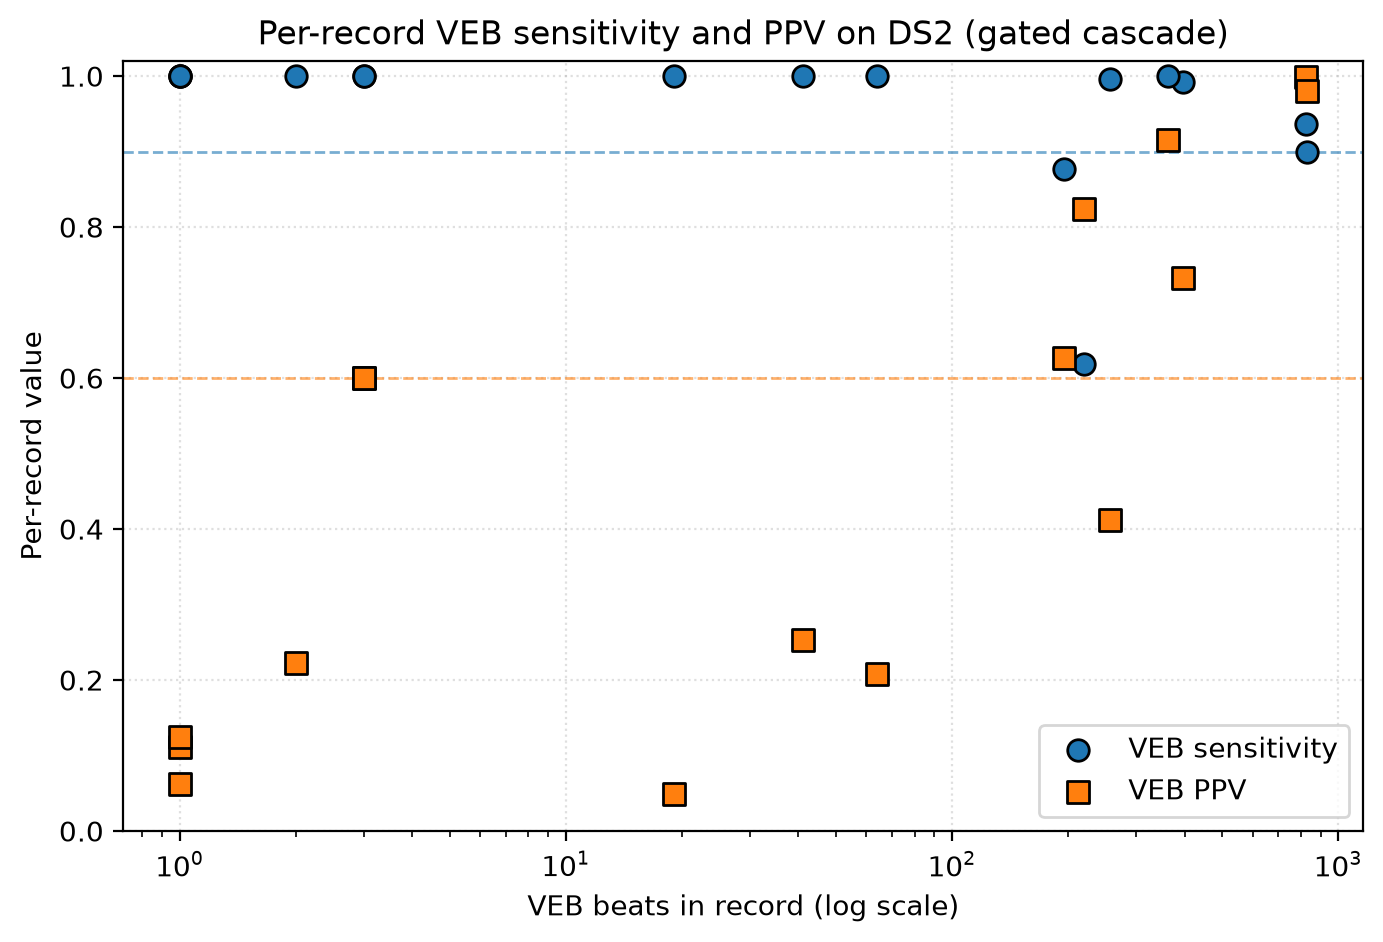
\includegraphics[keepaspectratio]{figures/fig6_perrecord.png}}
\caption{Figure 6}
\end{figure}

\textbf{Figure 6. Per-record robustness on DS2.} Per-record VEB
sensitivity (circles) and PPV (squares) on DS2 for the frozen gated
cascade, versus the record's VEB count (log scale). Dashed lines mark
the 0.90 sensitivity and 0.60 PPV targets. Only records with at least
one VEB beat are shown. Sensitivity is high and stable on the high-VEB
records except record 213; PPV is dispersed and falls well below target
on several low-VEB records.

\begin{figure}
\centering
\pandocbounded{\includegraphics[keepaspectratio]{figures/fig7_learningcurve.png}}
\caption{Figure 7}
\end{figure}

\textbf{Figure 7. Training-set-size learning curve.} DS2 VEB F1 (mean
with min-max band), sensitivity, and PPV versus DS1 training beats for
the single-stage model (T = 64, 2 seeds per point). In this limited
two-seed diagnostic sweep, additional DS1 data appeared to narrow seed
variance more than raise mean accuracy.

\subsection{5. Methods}\label{methods}

\subsubsection{5.1 Spike encoding}\label{spike-encoding}

Each 256-sample beat window is converted to a spike tensor by
count-pooled delta encoding. For each signal order in the set
\texttt{orders} (order 0 is the signal, order 1 its first difference),
threshold crossings of magnitude theta = 0.12 (in normalized signal
units) are accumulated into T time bins, producing two channels (rising
and falling crossings) per order. With \texttt{orders\ =\ {[}0,\ 1{]}}
this yields 2 x \textbar orders\textbar{} = 4 input channels over T
timesteps. Because crossings are pooled by count into bins, the total
number of input spikes over a beat is approximately conserved as T
varies; increasing T redistributes the same spikes into finer bins
rather than creating more of them (Section 8).

\subsubsection{5.2 Network}\label{network}

The classifier is a two-layer LIF network. A linear map \texttt{fc1}
projects the 4 input channels to H = 128 hidden LIF units; a linear map
\texttt{fc2} projects hidden spikes to 5 class logits. The three RR
features are projected once, through a separate dense map, into the
hidden state (they are not re-injected at every timestep). The readout
accumulates the output-layer membrane potential over T timesteps.
Training uses surrogate-gradient backpropagation-through-time (snnTorch
{[}Eshraghian2023{]}, following {[}Neftci2019{]}) with the Adam
optimizer, learning rate 4e-3, 100 epochs, batch size 512, and class
weights scaled as the square root of inverse class frequency to counter
imbalance. Unless stated otherwise the single-stage model uses T = 64.

\subsubsection{5.3 Operating point
selection}\label{operating-point-selection}

The network emits 5 logits; the decision adds a fixed per-class bias
vector \texttt{b\ =\ {[}0,\ b\_S,\ b\_V,\ b\_F,\ b\_Q{]}} and takes the
argmax, with \texttt{b\_F} and \texttt{b\_Q} set to a large negative
constant (-12) that strongly disfavours the fusion and unknown classes,
whose support in DS1 is too small to calibrate. This penalty makes those
predictions rare rather than impossible; a small residual of beats with
extreme logits still land there (Section 7.5), but they do not affect
the VEB-versus-rest decision. The two free parameters
\texttt{(b\_S,\ b\_V)} are selected by grid search on the validation
holdout only, and then frozen. We define three selection strategies:

\begin{itemize}
\tightlist
\item
  \textbf{sens-first:} maximize validation VEB PPV subject to validation
  VEB sensitivity at or above 0.90;
\item
  \textbf{ppv-first:} maximize validation VEB sensitivity subject to
  validation VEB PPV at or above 0.60;
\item
  \textbf{balanced:} maximize validation VEB F1.
\end{itemize}

When a strategy's constraint is infeasible on validation for a given
seed, we report that seed as infeasible rather than substituting a
degenerate maximum- sensitivity point. The single-stage NeuroBeat-VEB
uses sens-first, because missing ventricular beats is the more costly
error; we also report the full frontier so the tradeoff is explicit.

\subsubsection{5.4 Energy proxy: SynOps per
beat}\label{energy-proxy-synops-per-beat}

We report a per-beat synaptic-operation count, defined as the number of
accumulate operations triggered by spikes across the forward pass:

\texttt{SynOps\ =\ (sum\ over\ T\ of\ input\_spikes)\ *\ H\ +\ (sum\ over\ T\ of\ hidden\_spikes)\ *\ C\ +\ n\_RR\ *\ H},

where H = 128, C = 5, n\_RR = 3, and \texttt{input\_spikes} /
\texttt{hidden\_spikes} are the per-timestep active-unit counts. The
first term (input to hidden) dominates and is encoding-dependent, which
is why sparse, low-order input matters more than T. This proxy counts
the accumulate operations a neuromorphic core performs; it excludes
membrane-state updates, on-chip memory movement, the encoding and sensor
front end, and any host overhead. It is therefore a compute proxy and
not a measured energy figure (Sections 8 and 9). The budget throughout
is 25,000 SynOps/beat.

\textbf{On the choice of 25,000 SynOps/beat.} This budget is a fixed
design constraint we set before the final locked evaluation, not a
measured device figure and not a clinically validated energy threshold.
It is an exploratory, deployment-inspired target chosen to make the
design problem non-trivial in both directions: it sits below the cost of
running the full five-seed ensemble on every beat (about 71,000
SynOps/beat, Section 7.7), so ``ensemble everything'' is deliberately
out of budget and accuracy must instead be earned through sparsity and
gating; and it sits comfortably above the cheapest useful single-stage
model (about 14,000 SynOps/beat), so the budget is not satisfied by
default. Because every configuration in the paper is held to the same
number, the budget functions as a common yardstick for comparing designs
rather than as a guarantee about any particular chip. As a rough sense
of scale only, at roughly 100,000 beats per day a 25,000-SynOp/beat
detector performs on the order of a few billion spike-triggered
accumulates per day; we give this for intuition and do not translate it
into battery life, which depends on the hardware factors enumerated in
Section 9.

\subsubsection{5.5 Two-stage gated-ensemble
cascade}\label{two-stage-gated-ensemble-cascade}

A single model cannot reach both target thresholds at one operating
point (Section 7.1). We therefore route inference through two stages:

\begin{itemize}
\tightlist
\item
  \textbf{Screener (every beat).} A deliberately sparse LIF network (T =
  32, H = 64, encoding threshold 0.18, \texttt{orders\ =\ {[}0,\ 1{]}}),
  with its operating point fit on validation for high VEB recall. Its
  sparsity, not its shorter T, is what makes it cheap (Section 8):
  higher threshold and fewer hidden units reduce spike counts, whereas
  reducing T alone would not (Section 5.1).
\item
  \textbf{Confirmer (flagged beats only).} A three-seed ensemble of the
  T = 64 models already trained for the single-stage study, combined by
  logit averaging. It runs only on beats the screener flags. A beat is
  declared VEB if and only if both the screener and the ensemble
  confirmer fire.
\end{itemize}

Both operating points are fit on validation only (screener recall target
0.97; confirmer maximizes cascade VEB PPV subject to cascade VEB
sensitivity at or above 0.90 on validation), then frozen. Average energy
is

\texttt{SynOps(screener)\ +\ flag\_rate\ *\ K\ *\ SynOps(one\ confirmer\ member\ on\ flagged\ beats)},

with K = 3. Because the flag rate is small, the heavier confirmer
contributes little on average. The confirmer members' SynOps are
measured on the flagged (ectopic-enriched) beats, which are more active
and therefore more expensive per beat than an average DS2 beat; we use
that higher figure rather than the DS2-wide average, so the reported
energy is not optimistic.

\subsubsection{5.6 Seeds and model
selection}\label{seeds-and-model-selection}

Each configuration is trained with 5 seeds. For the single-stage frozen
artifact, the seed is chosen by validation VEB F1 among seeds that
satisfy the sens-first validation constraint, never by any DS2 or
external number. For the cascade, the confirmer uses seeds 0 to 2; we
report robustness to this choice in Section 7.3.

\subsubsection{5.7 Hyperparameter selection and
locking}\label{hyperparameter-selection-and-locking}

For transparency about what was tuned and what was not: the encoding and
architecture settings were fixed during exploratory development on DS1
and its validation holdout, guided by validation VEB F1 and SynOps,
before the final locked evaluation. This applies to the single-stage
settings (T = 64, H = 128, encoding threshold 0.12, orders {[}0, 1{]}),
the screener settings (T = 32, H = 64, threshold 0.18), the three-seed
confirmer, the 25,000-SynOps budget, and the choice of DS1 records 201,
207, and 223 as the validation holdout. This exploration was informal
rather than an exhaustive grid search, and we do not claim these values
are optimal; several of them (in particular H, the number of confirmer
seeds, and the exact encoding thresholds) were set to reasonable values
and not swept to convergence. A systematic sweep could plausibly improve
the operating points and is left as future work.

What we do guarantee is the locking discipline. Once these settings were
fixed, all operating points (single-stage and both cascade stages) were
fit only on the DS1 validation holdout, and every number reported on
DS2, SVDB, and INCART was produced by evaluating the resulting frozen
artifacts against test sets that played no role in any selection
(Section 6). The distinction we ask the reader to keep is between the
architecture and hyperparameters, which were set during development and
may be improvable, and the operating point and test evaluation, which
are strictly locked and are the basis for every headline claim.

\subsection{6. Evaluation protocol (no-leakage
statement)}\label{evaluation-protocol-no-leakage-statement}

To state precisely what is and is not controlled:

\begin{enumerate}
\def\labelenumi{\arabic{enumi}.}
\tightlist
\item
  The operating point (per-class biases), seed selection, decision
  threshold, and early-stopping decisions are fit only on the DS1
  validation holdout, never on DS2, SVDB, or INCART. This is enforced in
  code: the selection routines see only validation logits.
\item
  All operating points (single-stage and both cascade stages) are
  selected only on the DS1 validation holdout (records 201, 207, 223),
  which is patient-disjoint from DS1 training.
\item
  SVDB and INCART are test-only. No external beat enters training or
  operating- point selection for the VEB models. Every cross-database
  number uses the same frozen operating point selected on DS1
  validation.
\item
  Final reported artifacts and operating points were frozen before the
  final reported test tables were generated, and no test table was
  revised afterward to improve a number. We claim leakage-free
  operating-point and seed selection (points 1 to 3), not a fully
  blinded research process: the architecture and hyperparameters
  (Section 5.7) were set during exploratory development that was not
  blind to DS2, as is normal for method development. The guarantee is
  therefore that no reported operating point or seed was tuned on a test
  set, not that the process never observed DS2.
\end{enumerate}

The one deliberate exception is the SVEB specialist (Section 7.9), which
by design adds SVDB and INCART beats to training as an augmentation
study; its DS2 test set remains untouched, and we flag its non-standard
training explicitly. Because that specialist trains on SVDB and INCART,
its SVDB and INCART numbers are in-domain and diagnostic, not external
validation, and we label them as such (Section 7.9).

\subsection{7. Results}\label{results}

All results use 5 training seeds. We report seed mean with {[}min,
max{]} where a distribution exists, and 95\% bootstrap confidence
intervals (2,000 resamples over DS2 beats) for the headline cascade. DS2
contains 3,220 VEB beats out of 49,693 (Table 1), so a one-point change
in sensitivity corresponds to about 32 beats.

\subsubsection{7.1 Single-stage VEB
detection}\label{single-stage-veb-detection}

DS2 VEB detection under each validation-fit strategy (5 seeds), with
SynOps/beat, is given in Table 2.

\textbf{Table 2. Single-stage DS2 VEB detection under each
validation-fit operating-point strategy (5 seeds); seed mean with
{[}min, max{]}.}

\begin{longtable}[]{@{}
  >{\raggedright\arraybackslash}p{(\linewidth - 8\tabcolsep) * \real{0.2000}}
  >{\raggedright\arraybackslash}p{(\linewidth - 8\tabcolsep) * \real{0.2000}}
  >{\raggedright\arraybackslash}p{(\linewidth - 8\tabcolsep) * \real{0.2000}}
  >{\raggedright\arraybackslash}p{(\linewidth - 8\tabcolsep) * \real{0.2000}}
  >{\raggedright\arraybackslash}p{(\linewidth - 8\tabcolsep) * \real{0.2000}}@{}}
\toprule\noalign{}
\begin{minipage}[b]{\linewidth}\raggedright
Operating point
\end{minipage} & \begin{minipage}[b]{\linewidth}\raggedright
VEB sensitivity
\end{minipage} & \begin{minipage}[b]{\linewidth}\raggedright
VEB PPV
\end{minipage} & \begin{minipage}[b]{\linewidth}\raggedright
F1
\end{minipage} & \begin{minipage}[b]{\linewidth}\raggedright
SynOps/beat
\end{minipage} \\
\midrule\noalign{}
\endhead
\bottomrule\noalign{}
\endlastfoot
sens-first & 0.905 {[}0.878, 0.928{]} & 0.539 {[}0.490, 0.627{]} & 0.68
& about 14,300 \\
balanced & 0.857 {[}0.790, 0.912{]} & 0.679 {[}0.517, 0.780{]} & 0.76 &
about 14,300 \\
ppv-first & 0.845 {[}0.771, 0.888{]} & 0.700 {[}0.583, 0.791{]} & 0.77 &
about 14,300 \\
\end{longtable}

A single operating point buys sensitivity or precision, not both: at
sensitivity near 0.90 the PPV is about 0.54, and reaching PPV near 0.68
costs roughly 4 to 7 points of sensitivity. All single-stage
configurations sit under the SynOps budget. Note that the balanced point
has a higher F1 (0.76) than the cascade below (0.74): the cascade is not
F1-optimal, it is selected to satisfy both clinical thresholds
(sensitivity at or above 0.90 and PPV at or above 0.60) jointly, which
the balanced point does not (its sensitivity is 0.857).

\textbf{Frontier (Figure 2).} Sweeping the VEB decision threshold on DS2
(an oracle sweep, shown only to characterize what is achievable, not as
an operating point), the DS2 VEB PPV attainable at each sensitivity
level spans, across the 5 seeds, the ranges in Table 3.

\textbf{Table 3. DS2 VEB PPV attainable at each sensitivity level under
an oracle DS2 threshold sweep (range across 5 seeds). Shown to
characterize what is achievable, not used as an operating point.}

\begin{longtable}[]{@{}
  >{\raggedright\arraybackslash}p{(\linewidth - 8\tabcolsep) * \real{0.2000}}
  >{\raggedright\arraybackslash}p{(\linewidth - 8\tabcolsep) * \real{0.2000}}
  >{\raggedright\arraybackslash}p{(\linewidth - 8\tabcolsep) * \real{0.2000}}
  >{\raggedright\arraybackslash}p{(\linewidth - 8\tabcolsep) * \real{0.2000}}
  >{\raggedright\arraybackslash}p{(\linewidth - 8\tabcolsep) * \real{0.2000}}@{}}
\toprule\noalign{}
\begin{minipage}[b]{\linewidth}\raggedright
Sensitivity floor
\end{minipage} & \begin{minipage}[b]{\linewidth}\raggedright
0.80
\end{minipage} & \begin{minipage}[b]{\linewidth}\raggedright
0.85
\end{minipage} & \begin{minipage}[b]{\linewidth}\raggedright
0.90
\end{minipage} & \begin{minipage}[b]{\linewidth}\raggedright
0.92
\end{minipage} \\
\midrule\noalign{}
\endhead
\bottomrule\noalign{}
\endlastfoot
VEB PPV (range) & 0.57 to 0.78 & 0.57 to 0.69 & 0.56 to 0.65 & 0.48 to
0.57 \\
\end{longtable}

Two of the five seeds cannot exceed 0.90 sensitivity on DS2 even at the
oracle threshold, and no seed offers a single point at both sensitivity
at or above 0.90 and PPV at or above 0.60 with margin. This motivates
the cascade.

\subsubsection{7.2 Cross-database generalization
(single-stage)}\label{cross-database-generalization-single-stage}

A note on Table 2 versus Table 4, which report different quantities.
Table 2 gives 5-seed means (sens-first: 0.905 / 0.539 on DS2). Table 4
reports the single frozen artifact selected for cross-database testing,
chosen by validation VEB F1 among the sens-first-feasible seeds (Section
5.6); that artifact scored 0.894 / 0.490 on DS2. The frozen single-stage
model (sens-first, fit on DS1 validation) applied unchanged is reported
in Table 4.

\textbf{Table 4. Frozen single-stage cross-database VEB detection (one
operating point fit on DS1 validation, applied unchanged to all three
databases).}

\begin{longtable}[]{@{}lrrll@{}}
\toprule\noalign{}
Database & Beats & VEB beats & VEB sensitivity & VEB PPV \\
\midrule\noalign{}
\endhead
\bottomrule\noalign{}
\endlastfoot
MIT-BIH DS2 & 49,693 & 3,220 & 0.894 & 0.490 \\
MIT-BIH SVDB & 184,520 & 9,941 & 0.892 & 0.361 \\
INCART & 175,811 & 20,006 & 0.880 & 0.736 \\
\end{longtable}

VEB sensitivity holds in a narrow band (0.88 to 0.89) across three
databases with different patients, leads, and original sampling rates,
under one frozen operating point. PPV varies with class prevalence: it
is lower on the supraventricular-dense SVDB (more non-VEB beats
resembling VEB) and higher on the VEB-dense INCART. This is the expected
behaviour of a fixed threshold under prevalence shift and is why we
report sensitivity and PPV separately rather than a single accuracy
figure.

\subsubsection{7.3 Two-stage gated-ensemble
cascade}\label{two-stage-gated-ensemble-cascade-1}

The frozen cascade (screener recall target 0.97; confirmer fit for
cascade PPV subject to cascade sensitivity at or above 0.90; both on
validation only) is reported in Table 5.

\textbf{Table 5. Frozen gated-ensemble cascade cross-database VEB
detection (both stages' operating points fit on DS1 validation, then
frozen).}

\begin{longtable}[]{@{}lrrlll@{}}
\toprule\noalign{}
Database & Beats & VEB beats & VEB sensitivity & VEB PPV & Flag rate \\
\midrule\noalign{}
\endhead
\bottomrule\noalign{}
\endlastfoot
MIT-BIH DS2 & 49,693 & 3,220 & 0.923 & 0.616 & 0.271 \\
MIT-BIH SVDB & 184,520 & 9,941 & 0.904 & 0.377 & 0.345 \\
INCART & 175,811 & 20,006 & 0.901 & 0.835 & 0.241 \\
\end{longtable}

We report two bootstrap intervals for the DS2 point estimates. A
beat-level bootstrap (resampling beats independently, 2,000 resamples)
gives sensitivity {[}0.914, 0.932{]} and PPV {[}0.602, 0.630{]}. A
patient-level bootstrap (resampling the 22 DS2 records with replacement,
which respects within-record correlation) gives much wider intervals:
sensitivity {[}0.850, 0.976{]} and PPV {[}0.355, 0.814{]}. The gap
between the two is large because VEB beats are concentrated in a
minority of records, so a few patients dominate the estimate. The
patient-level interval is the honest one to quote: the point estimates
meet the targets on DS2's specific patient composition, but per-patient
behaviour varies substantially, and a wider prospective evaluation would
be needed to tighten this. Average energy on DS2 is
\texttt{5,987\ +\ 0.271\ *\ 3\ *\ 21,433\ =\ 23,385} SynOps/beat, within
the 25,000 budget. Robustness to the confirmer composition: ensembles of
K in \{2, 3, 5\} members and different 3-member subsets all give DS2
sensitivity at or above 0.90 at PPV between 0.59 and 0.64.

\subsubsection{7.4 Per-record robustness}\label{per-record-robustness}

Aggregate DS2 metrics can hide the fact that ventricular beats are
unevenly distributed across patients: two records (200 and 233) hold
1,656 of the 3,220 DS2 VEB beats (51\%), so the headline sensitivity is
effectively an average dominated by a few patients. Because a deployed
device sees one patient at a time, per-record behaviour is the more
deployment-relevant view. Table 6 gives the frozen cascade's per-record
VEB result for the 16 DS2 records that contain at least one VEB beat;
Figure 6 plots the same per-record sensitivity and PPV against each
record's VEB count.

\textbf{Table 6. Per-record DS2 VEB detection (frozen gated cascade),
for the 16 records with at least one VEB beat, sorted by VEB count.}
TP/FN/FP are beat counts; sensitivity = TP/(TP+FN); PPV = TP/(TP+FP).

\begin{longtable}[]{@{}lrrrrrr@{}}
\toprule\noalign{}
Record & VEB beats & TP & FN & FP & Sensitivity & PPV \\
\midrule\noalign{}
\endhead
\bottomrule\noalign{}
\endlastfoot
233 & 830 & 746 & 84 & 15 & 0.899 & 0.980 \\
200 & 826 & 774 & 52 & 1 & 0.937 & 0.999 \\
221 & 396 & 393 & 3 & 143 & 0.992 & 0.733 \\
228 & 362 & 362 & 0 & 33 & 1.000 & 0.916 \\
214 & 256 & 255 & 1 & 364 & 0.996 & 0.412 \\
213 & 220 & 136 & 84 & 29 & 0.618 & 0.824 \\
210 & 195 & 171 & 24 & 102 & 0.877 & 0.626 \\
219 & 64 & 64 & 0 & 243 & 1.000 & 0.208 \\
105 & 41 & 41 & 0 & 121 & 1.000 & 0.253 \\
202 & 19 & 19 & 0 & 369 & 1.000 & 0.049 \\
123 & 3 & 3 & 0 & 2 & 1.000 & 0.600 \\
234 & 3 & 3 & 0 & 2 & 1.000 & 0.600 \\
231 & 2 & 2 & 0 & 7 & 1.000 & 0.222 \\
100 & 1 & 1 & 0 & 8 & 1.000 & 0.111 \\
111 & 1 & 1 & 0 & 7 & 1.000 & 0.125 \\
121 & 1 & 1 & 0 & 15 & 1.000 & 0.062 \\
\end{longtable}

The six remaining DS2 records contain no VEB beats and so contribute
only false positives: 389 in total, which is 21\% of all 1,850 DS2 false
positives. Record 222 alone emits 252 and record 113 emits 116.

\textbf{Interpretation.} Three patterns bear on how much weight the
headline deserves. (i) Sensitivity is carried by the two largest
records: 200 (0.937) and 233 (0.899) supply half the VEB beats between
them, so the aggregate 0.923 would move materially if either behaved
differently. (ii) One record is genuinely weak: record 213 has 220 VEB
beats at sensitivity 0.618 and alone accounts for 84 of the 248 total
missed beats (34\%), a concentration that a beat-pooled metric obscures.
(iii) PPV is highly non-uniform, ranging from about 0.05 to 0.999 across
records; it is dragged down by a handful of records that emit many false
positives relative to their VEB count (202, 214, 219, 105) and by the
six VEB-free records. The headline PPV of 0.616 is therefore a
prevalence-weighted average, not a value the detector attains on a
typical single patient. This per-record dispersion is the concrete
reason the patient-level bootstrap interval (Section 7.3) is so much
wider than the beat-level one, and it is why we do not present the
aggregate as a per-patient guarantee.

\subsubsection{7.5 Error composition}\label{error-composition}

To show which classes the detector confuses with VEB, Table 7 gives the
VEB-versus-rest confusion for the frozen cascade on all three databases,
with each false positive attributed to the true AAMI class of the beat
that produced it. Table 8 gives the full five-class AAMI confusion for
the single-stage model on DS2.

\textbf{Table 7. VEB-versus-rest confusion for the frozen gated cascade,
with false positives broken down by the true class of the beat.} TN is
all correctly-rejected non-VEB beats.

\begin{longtable}[]{@{}
  >{\raggedright\arraybackslash}p{(\linewidth - 16\tabcolsep) * \real{0.0857}}
  >{\raggedleft\arraybackslash}p{(\linewidth - 16\tabcolsep) * \real{0.1143}}
  >{\raggedleft\arraybackslash}p{(\linewidth - 16\tabcolsep) * \real{0.1143}}
  >{\raggedleft\arraybackslash}p{(\linewidth - 16\tabcolsep) * \real{0.1143}}
  >{\raggedleft\arraybackslash}p{(\linewidth - 16\tabcolsep) * \real{0.1143}}
  >{\raggedleft\arraybackslash}p{(\linewidth - 16\tabcolsep) * \real{0.1143}}
  >{\raggedleft\arraybackslash}p{(\linewidth - 16\tabcolsep) * \real{0.1143}}
  >{\raggedleft\arraybackslash}p{(\linewidth - 16\tabcolsep) * \real{0.1143}}
  >{\raggedleft\arraybackslash}p{(\linewidth - 16\tabcolsep) * \real{0.1143}}@{}}
\toprule\noalign{}
\begin{minipage}[b]{\linewidth}\raggedright
Database
\end{minipage} & \begin{minipage}[b]{\linewidth}\raggedleft
TP
\end{minipage} & \begin{minipage}[b]{\linewidth}\raggedleft
FN
\end{minipage} & \begin{minipage}[b]{\linewidth}\raggedleft
FP
\end{minipage} & \begin{minipage}[b]{\linewidth}\raggedleft
TN
\end{minipage} & \begin{minipage}[b]{\linewidth}\raggedleft
FP: N
\end{minipage} & \begin{minipage}[b]{\linewidth}\raggedleft
FP: SVEB
\end{minipage} & \begin{minipage}[b]{\linewidth}\raggedleft
FP: F
\end{minipage} & \begin{minipage}[b]{\linewidth}\raggedleft
FP: Q
\end{minipage} \\
\midrule\noalign{}
\endhead
\bottomrule\noalign{}
\endlastfoot
MIT-BIH DS2 & 2,972 & 248 & 1,850 & 44,623 & 1,610 & 227 & 9 & 4 \\
MIT-BIH SVDB & 8,990 & 951 & 14,854 & 159,725 & 9,032 & 5,772 & 4 &
46 \\
INCART & 18,020 & 1,986 & 3,565 & 152,240 & 2,758 & 747 & 58 & 2 \\
\end{longtable}

\textbf{Table 8. Single-stage DS2 five-class AAMI confusion matrix
(frozen seed, sens-first operating point). Rows are true class, columns
are predicted class.} The fusion (F) and unknown (Q) columns carry a
large negative bias (Section 5.3), which strongly disfavours those
predictions rather than forbidding them: 718 beats (1.4\% of DS2) with
extreme logits still fall into the F and Q columns. Because the task is
VEB-versus-rest, these do not affect the VEB sensitivity or PPV.

\begin{longtable}[]{@{}lrrrrr@{}}
\toprule\noalign{}
True ~Pred & N & SVEB & VEB & F & Q \\
\midrule\noalign{}
\endhead
\bottomrule\noalign{}
\endlastfoot
N & 39,970 & 1,059 & 2,752 & 163 & 297 \\
SVEB & 1,154 & 222 & 221 & 0 & 240 \\
VEB & 284 & 55 & 2,880 & 1 & 0 \\
F & 347 & 0 & 24 & 17 & 0 \\
Q & 3 & 0 & 4 & 0 & 0 \\
\end{longtable}

\textbf{What the errors are made of.} On DS2, false positives are
dominated by normal beats (1,610 of 1,850, 87\%), with a smaller but
non-trivial supraventricular contribution (227, 12\%); fusion and
unknown contribute few VEB false positives. The single-stage matrix
(Table 8) locates the same effect at the class level: the largest
off-diagonal entry into the VEB column is N-to-VEB (2,752 beats), and
221 true SVEB beats are also read as VEB, consistent with single-lead
morphological overlap between aberrantly-conducted supraventricular
beats and ventricular ectopy. This overlap is what makes the SVDB PPV
drop: on the supraventricular-dense SVDB, 5,772 of the 14,854 false
positives (39\%) are true SVEB beats, a far larger share than on DS2
(12\%) or INCART (21\%). The database with the most supraventricular
beats produces the most SVEB-to-VEB confusion, so the lower SVDB PPV
reflects class composition and single-lead ambiguity rather than a
change in the detector's ventricular behaviour, whose sensitivity is
stable across all three databases (Section 7.3).

\subsubsection{7.6 Statistical comparison}\label{statistical-comparison}

To test whether the cascade's improvement over simpler configurations
exceeds DS2 sampling noise, we use a paired record-level bootstrap: we
resample the 22 DS2 records with replacement (2,000 resamples,
respecting within-record correlation) and, on each resample, recompute
the VEB F1 of two systems evaluated at their own frozen operating
points, reporting the distribution of the paired difference. This is the
record-level analogue of the interval in Section 7.3 and is stricter
than a beat-level test because it does not treat beats from one patient
as independent.

\textbf{Table 9. Paired record-level bootstrap on DS2 (2,000 resamples).
Difference in VEB F1, gated cascade minus the comparator; positive
favours the cascade.} ``Cascade better'' is the fraction of resamples in
which the cascade's F1 is higher.

\begin{longtable}[]{@{}
  >{\raggedright\arraybackslash}p{(\linewidth - 6\tabcolsep) * \real{0.2000}}
  >{\raggedleft\arraybackslash}p{(\linewidth - 6\tabcolsep) * \real{0.2667}}
  >{\raggedleft\arraybackslash}p{(\linewidth - 6\tabcolsep) * \real{0.2667}}
  >{\raggedleft\arraybackslash}p{(\linewidth - 6\tabcolsep) * \real{0.2667}}@{}}
\toprule\noalign{}
\begin{minipage}[b]{\linewidth}\raggedright
Comparison
\end{minipage} & \begin{minipage}[b]{\linewidth}\raggedleft
Median F1 difference
\end{minipage} & \begin{minipage}[b]{\linewidth}\raggedleft
95\% interval
\end{minipage} & \begin{minipage}[b]{\linewidth}\raggedleft
Cascade better
\end{minipage} \\
\midrule\noalign{}
\endhead
\bottomrule\noalign{}
\endlastfoot
Cascade vs single-stage (sens-first) & +0.103 & {[}+0.060, +0.142{]} &
100\% \\
Cascade vs full 5-seed ensemble (every beat) & +0.013 & {[}-0.003,
+0.027{]} & 95\% \\
\end{longtable}

The cascade's advantage over the single-stage model is large and
consistent: its F1 is higher in every one of the 2,000 record resamples
and the interval excludes zero by a wide margin. Against the full
five-seed ensemble that runs on every beat, the cascade is statistically
indistinguishable in F1 (the interval includes zero) while using roughly
a third of the operations (Section 7.7); the gating therefore buys the
energy reduction at no measurable accuracy cost, which is the paper's
central efficiency claim. We run the same paired test against the
non-spiking baselines in Section 7.8 (Table 12); to preview the honest
outcome, the cascade is ahead of the CNN and linear SVM but behind the
TCN, ResNet-lite, and gradient-boosted-tree baselines on DS2 F1, which
we report rather than obscure. We give no p-values: at 22 patients the
bootstrap interval and the fraction of resamples favouring each system
are the summaries we consider defensible.

\subsubsection{7.7 Accuracy-energy Pareto (Figure
3)}\label{accuracy-energy-pareto-figure-3}

DS2 accuracy against per-beat compute for the main configurations is
given in Table 10.

\textbf{Table 10. Accuracy-energy operating points on DS2. SNN rows are
SynOps/beat; the dense-baseline comparison is in Table 11.}

\begin{longtable}[]{@{}
  >{\raggedright\arraybackslash}p{(\linewidth - 4\tabcolsep) * \real{0.3333}}
  >{\raggedright\arraybackslash}p{(\linewidth - 4\tabcolsep) * \real{0.3333}}
  >{\raggedright\arraybackslash}p{(\linewidth - 4\tabcolsep) * \real{0.3333}}@{}}
\toprule\noalign{}
\begin{minipage}[b]{\linewidth}\raggedright
Model
\end{minipage} & \begin{minipage}[b]{\linewidth}\raggedright
DS2 sens / PPV
\end{minipage} & \begin{minipage}[b]{\linewidth}\raggedright
Compute/beat
\end{minipage} \\
\midrule\noalign{}
\endhead
\bottomrule\noalign{}
\endlastfoot
Single-stage (sens-first) & 0.894 / 0.490 & 14,200 SynOps \\
Naive T32 cascade & 0.883 / 0.622 & 19,400 SynOps \\
Full 5-seed ensemble (every beat) & 0.932 / 0.595 & about 71,000
SynOps \\
Gated-ensemble cascade & 0.923 / 0.616 & 23,385 SynOps \\
\end{longtable}

The full ensemble reaches the target corner but costs about five forward
passes and exceeds the budget. The gated cascade recovers most of that
accuracy within budget by running the ensemble only on flagged beats.
The naive T32 cascade is a cautionary point: it costs more than the
single-stage model, because a shorter network is not a cheaper one under
count-pooled encoding (Section 8).

\subsubsection{7.8 Non-spiking baselines on the same
split}\label{non-spiking-baselines-on-the-same-split}

We train 1-D CNN and LSTM baselines under the identical protocol: same
DS1 train, same beat-plus-RR inputs, same validation-locked sens-first
operating point, same frozen DS2 test, 5 seeds (Table 11).

\textbf{Table 11. Non-spiking baselines under the identical
validation-locked protocol. Operation units differ (SynOps vs MACs) and
are not directly comparable, as discussed below.}

\begin{longtable}[]{@{}lllll@{}}
\toprule\noalign{}
Model & DS2 sens & DS2 PPV & Operations/beat & Params \\
\midrule\noalign{}
\endhead
\bottomrule\noalign{}
\endlastfoot
CNN (1-D, beat+RR) & 0.945 {[}0.926, 0.959{]} & 0.434 & 356k MACs &
2.9k \\
LSTM (beat+RR) & 0.940 {[}0.911, 0.974{]} & 0.178 & 4.26M MACs &
17.5k \\
SNN single-stage & 0.894 & 0.490 & 14.2k SynOps & 18k \\
SNN gated-ensemble & 0.923 & 0.616 & 23.4k SynOps & n/a \\
\end{longtable}

Two observations. First, the dense baselines show the same
sensitivity/precision tradeoff: under the sens-first operating point
they reach high sensitivity (about 0.94) but low PPV (0.43 for the CNN,
0.18 for the LSTM), so the tradeoff is a property of single-lead VEB
detection rather than of spiking networks. Second, on operation count
the SNN is far lower: 14k to 23k SynOps versus 356k (CNN) and 4.26M
(LSTM) MACs. We state this carefully. A SynOp (a spike-triggered
accumulate) and a MAC (a multiply-accumulate) are not the same unit, and
this comparison is an operation-count advantage under a proxy model, not
a measured energy ratio. We add stronger baselines below (Table 12);
measured microcontroller energy remains the key missing piece (Section
9).

Post-training int8 weight quantization of the CNN (per-tensor symmetric,
weights only, activations left in float, 3 seeds) preserves DS2 VEB
detection: fp32 0.951 / 0.417 versus int8 0.951 / 0.444 (sensitivity /
PPV), with weight memory reduced from 11.6 kB to 3.1 kB. This is the
fair embedded operating point for the dense baseline: the MAC count is
unchanged (356k/beat), but an int8 MAC is materially cheaper and smaller
than an fp32 MAC on typical microcontrollers. Quantization therefore
closes part of the compute gap in energy-per-operation terms without
changing the operation count, and a full int8 pipeline (quantized
activations, with calibration) plus measured board energy is the natural
next comparison (Section 9).

\textbf{Stronger baselines, and an honest ranking.} To avoid overstating
the spiking model, we add stronger baselines under the identical
validation-locked protocol: a compact temporal convolutional network
(TCN), a ResNet-lite 1-D CNN, gradient-boosted trees on
morphology-plus-RR features, and a linear SVM (Table 12). Each neural
model is frozen at the seed with the best validation VEB F1; the
classical models use a fixed seed and a validation-locked VEB-vs-rest
threshold. The ``cascade minus model'' column is the paired record-level
bootstrap difference in DS2 VEB F1 (the same test as Section 7.6); a
negative value means the baseline beats the cascade.

\textbf{Table 12. Additional embedded baselines under the identical
protocol (frozen single artifact), with the gated cascade as reference.
F1 is the VEB F1 at the frozen operating point. ``Cascade minus model''
is the paired record-level bootstrap difference in DS2 VEB F1; negative
means the baseline is more accurate than the cascade.}

\begin{longtable}[]{@{}
  >{\raggedright\arraybackslash}p{(\linewidth - 10\tabcolsep) * \real{0.1667}}
  >{\raggedright\arraybackslash}p{(\linewidth - 10\tabcolsep) * \real{0.1667}}
  >{\raggedright\arraybackslash}p{(\linewidth - 10\tabcolsep) * \real{0.1667}}
  >{\raggedright\arraybackslash}p{(\linewidth - 10\tabcolsep) * \real{0.1667}}
  >{\raggedright\arraybackslash}p{(\linewidth - 10\tabcolsep) * \real{0.1667}}
  >{\raggedright\arraybackslash}p{(\linewidth - 10\tabcolsep) * \real{0.1667}}@{}}
\toprule\noalign{}
\begin{minipage}[b]{\linewidth}\raggedright
Model
\end{minipage} & \begin{minipage}[b]{\linewidth}\raggedright
DS2 VEB sens
\end{minipage} & \begin{minipage}[b]{\linewidth}\raggedright
DS2 VEB PPV
\end{minipage} & \begin{minipage}[b]{\linewidth}\raggedright
F1
\end{minipage} & \begin{minipage}[b]{\linewidth}\raggedright
Operations/beat
\end{minipage} & \begin{minipage}[b]{\linewidth}\raggedright
Cascade minus model F1 {[}95\% CI{]}
\end{minipage} \\
\midrule\noalign{}
\endhead
\bottomrule\noalign{}
\endlastfoot
Gated cascade (reference) & 0.923 & 0.616 & 0.739 & about 23.4k SynOps &
(reference) \\
TCN & 0.939 & 0.729 & 0.821 & about 1.02M MACs & -0.088 {[}-0.251,
+0.082{]} \\
ResNet-lite & 0.910 & 0.761 & 0.829 & about 539k MACs & -0.089
{[}-0.188, +0.009{]} \\
Gradient-boosted trees & 0.974 & 0.678 & 0.800 & about 200 trees (depth
4) & -0.060 {[}-0.146, +0.019{]} \\
Linear SVM & 0.981 & 0.259 & 0.410 & 259 MACs & +0.314 {[}+0.163,
+0.477{]} \\
\end{longtable}

For the gradient-boosted trees and SVM we report model structure rather
than an operation count: tree inference is dominated by branch,
comparison, and memory-access operations rather than
multiply-accumulates, so a fair embedded comparison of those models
would require measured latency or energy, not an operation count. The
result is a useful corrective. Three of these baselines reach higher DS2
VEB F1 than the gated cascade: the TCN (0.939 / 0.729), ResNet-lite
(0.910 / 0.761), and gradient-boosted trees (0.974 / 0.678); the paired
bootstrap puts the cascade ahead of them in only 14\%, 3\%, and 5\% of
record resamples, respectively. The cascade does clearly beat the
higher-sensitivity, lower-precision models: the fp32 and int8 CNN (ahead
in 98\% and 97\% of resamples) and the linear SVM (100\%). We therefore
do not claim the spiking cascade is the most accurate DS2 VEB detector;
on accuracy alone, a gradient-boosted tree on morphology-plus-RR
features and a compact TCN are both better. What separates the cascade
is per-beat operation count: it runs at about 23,000 SynOps/beat,
roughly 20 to 45 times below the TCN and ResNet-lite MAC counts, while
the tree and SVM models are non-spiking and do not map onto neuromorphic
hardware. Whether that operation-count gap translates into an energy
advantage depends on measured hardware energy, which we do not yet have
(Section 9); this comparison is exactly why we treat measured energy,
not the SynOps proxy, as the decisive missing experiment, and why we
confine the spiking contribution to the operation-count and
neuromorphic-suitability axis rather than to accuracy. (The
gradient-boosted-tree and SVM baselines use a binary VEB-vs-rest
operating point, a slightly more favourable mechanism than the
five-class bias used for the neural and spiking models; the TCN and
ResNet-lite, which also beat the cascade, use the identical five-class
mechanism.)

\subsubsection{7.9 Supraventricular beats: a single-lead negative
result}\label{supraventricular-beats-a-single-lead-negative-result}

Supraventricular ectopic beats often differ from normal beats mainly in
timing and subtle morphology, and DS1 contains few of them (Table 1). As
an incidental output of the VEB model, DS2 SVEB sensitivity is about
0.13; adding supraventricular-rich SVDB to training raises it to about
0.24, and a higher-time-resolution variant to about 0.27, all still low.

We then trained a dedicated SVEB specialist (higher time resolution,
SVDB and INCART added to training, an SVEB-first operating point, 5
seeds). It does not yield a usable detector (Table 13).

\textbf{Table 13. SVEB specialist on DS2 (non-standard training: SVDB
and INCART added to training; see text). ``Degraded'' indicates the VEB
class collapses at that regime.}

\begin{longtable}[]{@{}
  >{\raggedright\arraybackslash}p{(\linewidth - 6\tabcolsep) * \real{0.2500}}
  >{\raggedright\arraybackslash}p{(\linewidth - 6\tabcolsep) * \real{0.2500}}
  >{\raggedright\arraybackslash}p{(\linewidth - 6\tabcolsep) * \real{0.2500}}
  >{\raggedright\arraybackslash}p{(\linewidth - 6\tabcolsep) * \real{0.2500}}@{}}
\toprule\noalign{}
\begin{minipage}[b]{\linewidth}\raggedright
Seed regime
\end{minipage} & \begin{minipage}[b]{\linewidth}\raggedright
DS2 SVEB sens
\end{minipage} & \begin{minipage}[b]{\linewidth}\raggedright
DS2 SVEB PPV
\end{minipage} & \begin{minipage}[b]{\linewidth}\raggedright
DS2 VEB sens
\end{minipage} \\
\midrule\noalign{}
\endhead
\bottomrule\noalign{}
\endlastfoot
calibrated (seeds 0 to 2) & 0.16 to 0.27 & 0.07 to 0.15 & degraded \\
degenerate (seeds 3 to 4) & 0.82 to 0.94 & 0.04 to 0.06 & 0.18 to
0.24 \\
\end{longtable}

The high-sensitivity seeds reach it only by flagging almost all beats as
SVEB (PPV at or below 0.06), which collapses the ventricular class. DS2
SVEB PPV never exceeds about 0.15 at any operating point, and the
outcome is unstable across seeds.

\textbf{On the INCART result: in-domain, not external validation.} The
same specialist reaches SVEB sensitivity about 0.62 on 12-lead INCART.
This must not be read as external validation: INCART supraventricular
beats were part of this specialist's augmented training set, so the
INCART number is an in-domain, diagnostic observation. Read only as
diagnostic, it is consistent with the limiting factor being available
lead information rather than model capacity, since the 12-lead recording
appears to separate supraventricular beats more readily; but because the
beats are in-domain, it does not establish generalization and must not
be interpreted as cross-database SVEB performance. (This is the one
place in the paper where an external database enters training, and we
confine it to this diagnostic role; the DS2 SVEB test set remains
untouched.) We therefore treat single-lead SVEB as an open problem and,
importantly, do not allow it to reshape the VEB operating point.
Multi-lead input (MIT-BIH provides a second lead; supraventricular beats
separate better on some leads) and richer, genuinely held-out SVEB
validation data are the natural next steps (Section 9).

\subsubsection{7.10 End-to-end detection with detected
R-peaks}\label{end-to-end-detection-with-detected-r-peaks}

Every result so far assumes ground-truth R-peak locations. To test how
far that assumption carries, we ran the frozen cascade on DS2 with beats
segmented at DETECTED R-peaks and RR features recomputed from the
detected-peak spacing (no annotations at inference), scoring VEB
detection against the true labels so that a missed R-peak becomes an
end-to-end false negative and a spurious detection an end-to-end false
positive. We report two detectors: wfdb's standard XQRS detector and the
repository's minimal static-threshold on-patch detector (Table 14).

\textbf{Table 14. End-to-end DS2 VEB detection with detected (not
annotated) R-peaks. Beat sensitivity/PPV are for R-peak detection; the
last two columns are the frozen cascade scored against true labels
through each detector.}

\begin{longtable}[]{@{}
  >{\raggedright\arraybackslash}p{(\linewidth - 8\tabcolsep) * \real{0.1579}}
  >{\raggedleft\arraybackslash}p{(\linewidth - 8\tabcolsep) * \real{0.2105}}
  >{\raggedleft\arraybackslash}p{(\linewidth - 8\tabcolsep) * \real{0.2105}}
  >{\raggedleft\arraybackslash}p{(\linewidth - 8\tabcolsep) * \real{0.2105}}
  >{\raggedleft\arraybackslash}p{(\linewidth - 8\tabcolsep) * \real{0.2105}}@{}}
\toprule\noalign{}
\begin{minipage}[b]{\linewidth}\raggedright
Detector
\end{minipage} & \begin{minipage}[b]{\linewidth}\raggedleft
Beat sens
\end{minipage} & \begin{minipage}[b]{\linewidth}\raggedleft
Beat PPV
\end{minipage} & \begin{minipage}[b]{\linewidth}\raggedleft
End-to-end VEB sens
\end{minipage} & \begin{minipage}[b]{\linewidth}\raggedleft
End-to-end VEB PPV
\end{minipage} \\
\midrule\noalign{}
\endhead
\bottomrule\noalign{}
\endlastfoot
Annotated R-peaks (reference) & 1.000 & 1.000 & 0.923 & 0.616 \\
XQRS (standard) & 0.997 & 0.999 & 0.884 & 0.593 \\
Minimal on-patch detector & 0.784 & 1.000 & 0.513 & 0.479 \\
\end{longtable}

With a competent standard detector (XQRS, beat sensitivity 0.997), the
end-to-end cost is modest: VEB sensitivity falls from 0.923 to 0.884 and
PPV from 0.616 to 0.593. We state the practical consequence plainly:
under detected R-peaks the cascade falls below the 0.90 sensitivity
target that the annotation-based operating point meets, even though the
degradation with XQRS is small. Of the 3,220 true VEBs, 126 (3.9\%) are
missed because XQRS places no peak on them, a higher rate than its 0.3\%
overall beat-miss rate and consistent with ventricular beats being
harder to detect (wide, atypical QRS); the remainder of the drop is 247
detected-but-misclassified VEBs. The minimal on-patch detector tells the
other half of the story: its beat sensitivity is only 0.784 and
end-to-end VEB sensitivity collapses to 0.513. The R-peak stage is
therefore a first-order determinant of end-to-end performance: paired
with a competent detector the annotation-conditional headline degrades
gracefully, but a weak detector is catastrophic, so detector choice
cannot be treated as an afterthought.

\subsubsection{7.11 Sensitivity to training-set
size}\label{sensitivity-to-training-set-size}

To test whether the VEB result is limited by training-set size, we
retrained the single-stage model (T = 64, the paper configuration) on
stratified 10\%, 25\%, 50\%, and 100\% of DS1-train, fitting the
sens-first operating point on DS1-val and reporting frozen DS2 VEB
detection (2 seeds per point; Table 15, Figure 7). The data subset at a
given fraction is fixed, so only the training-set size varies.

\textbf{Table 15. DS2 VEB detection versus DS1 training-set size
(single-stage, T = 64, sens-first, 2 seeds; mean, with F1 min-max
band).}

\begin{longtable}[]{@{}
  >{\raggedright\arraybackslash}p{(\linewidth - 10\tabcolsep) * \real{0.1304}}
  >{\raggedleft\arraybackslash}p{(\linewidth - 10\tabcolsep) * \real{0.1739}}
  >{\raggedleft\arraybackslash}p{(\linewidth - 10\tabcolsep) * \real{0.1739}}
  >{\raggedleft\arraybackslash}p{(\linewidth - 10\tabcolsep) * \real{0.1739}}
  >{\raggedleft\arraybackslash}p{(\linewidth - 10\tabcolsep) * \real{0.1739}}
  >{\raggedleft\arraybackslash}p{(\linewidth - 10\tabcolsep) * \real{0.1739}}@{}}
\toprule\noalign{}
\begin{minipage}[b]{\linewidth}\raggedright
DS1 train used
\end{minipage} & \begin{minipage}[b]{\linewidth}\raggedleft
Train beats
\end{minipage} & \begin{minipage}[b]{\linewidth}\raggedleft
VEB beats
\end{minipage} & \begin{minipage}[b]{\linewidth}\raggedleft
DS2 sens
\end{minipage} & \begin{minipage}[b]{\linewidth}\raggedleft
DS2 PPV
\end{minipage} & \begin{minipage}[b]{\linewidth}\raggedleft
DS2 F1 {[}min, max{]}
\end{minipage} \\
\midrule\noalign{}
\endhead
\bottomrule\noalign{}
\endlastfoot
10\% & 4,458 & 291 & 0.920 & 0.425 & 0.563 {[}0.431, 0.695{]} \\
25\% & 11,144 & 727 & 0.850 & 0.544 & 0.659 {[}0.569, 0.748{]} \\
50\% & 22,287 & 1,454 & 0.897 & 0.494 & 0.627 {[}0.563, 0.692{]} \\
100\% & 44,573 & 2,907 & 0.926 & 0.526 & 0.670 {[}0.648, 0.693{]} \\
\end{longtable}

The curve is essentially flat. VEB sensitivity shows no upward trend
across the range (0.85 to 0.93), so even a tenth of DS1 (291 VEB beats)
reaches the sensitivity the full set reaches; the mean F1 rises from
10\% to 25\% of the data and then plateaus (0.659 at 25\% versus 0.670
at 100\%). What more data buys is not a higher mean but lower variance:
the F1 min-max band narrows from {[}0.431, 0.695{]} at 10\% to {[}0.648,
0.693{]} at 100\%, consistent with the calibration-variance account of
Sections 7.1 and 8. The single-stage VEB result is therefore saturated
with respect to DS1 training-set size: more same-distribution MIT-BIH
data would stabilize the operating point but is unlikely to raise
accuracy, which points back to architecture, encoding, and single-lead
information (Section 7.8) as the operative limits, not sample count.

\subsection{8. Discussion}\label{discussion}

\textbf{(a) Honest evaluation lowers headline numbers but increases
trust.} Freezing the operating point on validation rather than test, and
reporting inter-patient rather than intra-patient results, lowers our
headline metrics relative to test-tuned or intra-patient reports. The
compensating evidence is stability under a fixed decision rule: with one
frozen operating point, VEB sensitivity remained at or above 0.90 across
three databases, while PPV varied by database, which a threshold tuned
per test set would not demonstrate. We regard this frozen cross-database
behaviour as the most decision-relevant result in the paper.

\textbf{(b) Energy-accounted models need explicit budgets.} Reporting
SynOps for every configuration, and enforcing a fixed budget, changes
which design choices look attractive. It is what exposes the naive
cascade as a false economy and the full ensemble as over budget, and it
is what makes the sparse-screener design necessary rather than
incidental.

\textbf{(c) Time resolution is not the same as energy cost under
count-pooled encoding.} Because count-pooling approximately conserves
total input spikes across T, the dominant SynOps term is roughly
independent of T in our measurements. Two consequences follow under this
encoding: raising T can sharpen discrimination at little additional
energy cost, and a shorter network is not necessarily a cheaper one. A
screener is therefore made cheap by reducing channels, hidden units, or
spike rate (via a higher threshold), which is how our screener is built.

\textbf{(d) The cascade is consistent with reducing a
calibration-variance limit at low average cost.} The DS2 oracle frontier
shows that sensitivity at or above 0.90 at PPV at or above 0.60 is
attainable, yet single models calibrated on a small validation holdout
land there only occasionally and vary across seeds. A small ensemble
reduces model variance and appears to calibrate more stably, reaching
0.918 / 0.634 on DS2 for three members; gating it behind a sparse
screener delivers comparable accuracy within budget, and the paired
bootstrap (Section 7.6) confirms the cascade matches the full ensemble
in F1 at a fraction of the operations.

\textbf{(e) VEB is usable but not best-in-class on accuracy; single-lead
SVEB is not solved.} The VEB result is usable under a strict protocol
and an energy budget, but we do not claim it is the most accurate
detector: under the identical protocol a compact TCN, a ResNet-lite CNN,
and gradient-boosted trees reach higher DS2 F1 (Section 7.8). The
spiking model's case rests on per-beat operation count and neuromorphic
suitability, pending measured energy, not on accuracy leadership. The
SVEB result is a clean negative under the same protocol, and we present
it as such.

\textbf{Alternative explanations we cannot fully exclude.} The
cross-database PPV differences could reflect annotation-convention
differences between databases rather than only prevalence. The
single-model seed variance could partly reflect optimization noise
rather than only calibration; the ensemble would help in either case. We
report both beat-level and patient-level bootstrap intervals (Section
7.3); the patient-level interval is much wider because a few records
dominate the DS2 VEB count, and it is the interval we treat as the
honest uncertainty.

\subsection{9. Limitations}\label{limitations}

\begin{itemize}
\tightlist
\item
  \textbf{SynOps is an architecture-level compute proxy, not hardware
  energy.} The SynOps count is a property of the network and its spike
  statistics; it should be interpreted as a compute proxy and not as
  measured joules. Real energy on a device depends on the specific
  neuromorphic chip or microcontroller and its energy-per-operation,
  on-chip and off-chip memory movement (frequently the true bottleneck),
  the input-encoding pipeline, the compiler and runtime, the sensor
  front end and analog-to-digital conversion, the R-peak detection
  stage, and whether inference runs batched or streaming. We report no
  measured hardware energy, and the operation-count gap to the dense
  baselines (Section 7.8) is an operation-count difference under a
  proxy, not an energy ratio. Measuring end-to-end energy on both a
  microcontroller (for the quantized CNN) and a neuromorphic target (for
  the SNN) is the single most important addition for any hardware-energy
  claim and is our primary item of future work.
\item
  \textbf{Retrospective public data only.} All data are curated public
  research databases with expert beat annotations. Performance on raw,
  artefact-laden device recordings is untested.
\item
  \textbf{Small validation holdout.} Three DS1 records make single-model
  operating points noisy; the ensemble mitigates but does not remove
  this. A larger or cross-validated holdout is likely to tighten
  calibration. A training-set-size ablation (Section 7.11) shows that
  more training data narrows seed variance but does not raise DS2
  accuracy, so this noise is a holdout-size and calibration effect
  rather than a training-data-volume effect.
\item
  \textbf{Detection depends on the R-peak stage.} The headline numbers
  use provided annotations. An end-to-end ablation (Section 7.10) shows
  that swapping in a standard detector (XQRS) lowers VEB sensitivity/PPV
  modestly to 0.884 / 0.593, but a weak detector collapses them to 0.513
  / 0.479. A deployable system must include a competent R-peak detector,
  and its errors, especially missed ventricular beats, propagate to the
  end-to-end result.
\item
  \textbf{Prevalence-dependent PPV.} Cross-database PPV is sensitive to
  class composition, so PPV numbers should be read together with the
  beat counts.
\item
  \textbf{Single lead.} Results use one lead; SVEB in particular appears
  to need more lead information.
\item
  \textbf{Large between-patient variance.} With only 22 DS2 patients, a
  patient-level bootstrap gives wide intervals (VEB sensitivity 0.85 to
  0.98, PPV 0.36 to 0.81). The point estimates hold for DS2's
  composition, but per-patient behaviour varies substantially, so a
  larger prospective cohort is needed to tighten them.
\item
  \textbf{No prospective or clinical-workflow validation, and no
  subgroup or demographic fairness analysis.} Nothing here has been
  validated in a deployment or against regulatory-grade endpoints.
\end{itemize}

\subsection{10. Clinical and commercial
relevance}\label{clinical-and-commercial-relevance}

The most credible near-term role for this work is as a low-power VEB
screening component inside a larger pipeline: wearable or patch ECG,
Holter-style ambulatory monitoring, remote patient monitoring, or a
neuromorphic edge inference block that flags ventricular ectopy for
downstream review. In such a role, high sensitivity at a controlled
compute budget, with predictable cross-database behaviour, is the
relevant property. A PPV around 0.6 may be compatible with a screening
workflow in which flagged beats are reviewed downstream, but the
acceptable false-positive burden depends on the clinical setting and is
not established here.

We make no claim of diagnostic or product readiness, and the headline
experiment deliberately isolates the classifier by assuming
pre-annotated R-peak locations and clean, curated beats; Section 7.10
relaxes the first assumption and shows the end-to-end cost of the R-peak
stage is modest with a standard detector and severe with a weak one. A
deployable system would additionally require robust on-device R-peak
detection, rejection of unreadable or noise-corrupted segments,
motion-artifact handling, streaming (rather than whole-record batch)
inference, an explicit policy for uncertain or borderline beats,
patient-level summarization and reporting rather than per-beat labels,
integration into a clinical workflow with defined alarm handling,
measured energy on the target hardware, and quality-system,
software-as-a-medical-device, and regulatory validation. NeuroBeat as
evaluated here is therefore a candidate low-power component for such a
pipeline, not a complete or cleared product.

\subsection{11. Conclusion}\label{conclusion}

NeuroBeat is a deliberately compact and conventional spiking network;
its main contribution is not the architecture but the evaluation. Under
a validation-locked inter-patient protocol and an explicit per-beat
SynOps budget, a gated-ensemble cascade reaches 0.923 VEB sensitivity at
0.616 PPV on MIT-BIH DS2 within 23,385 SynOps/beat, and, under one
frozen operating point, keeps VEB sensitivity at or above 0.90 on two
unseen databases. The results come with clear boundaries: SynOps is a
compute proxy and not measured energy; PPV varies with database class
composition and is dispersed across patients, so a patient-level
bootstrap gives wide intervals; single-lead supraventricular detection
is reported as an unresolved negative result; and nothing here has been
clinically validated. Within those boundaries, the useful output is a
reusable pattern for reporting SNN-ECG work: lock the operating point on
validation, account for per-beat compute, freeze cross-database tests,
and report the per-patient and negative results rather than only the
headline. We release the protocol, the SynOps budgeting, and all
artifacts so that others can reuse and scrutinize them.

\subsection{12. Code and data
availability}\label{code-and-data-availability}

\begin{itemize}
\tightlist
\item
  \textbf{Code:} github.com/Talch87/neuro-beat (AGPL-3.0 / commercial
  dual license).
\item
  \textbf{Live results page:} talch87.github.io/neuro-beat.
\item
  \textbf{Data:} all databases are public on PhysioNet: the MIT-BIH
  Arrhythmia Database {[}Moody2001, Goldberger2000{]}, the MIT-BIH
  Supraventricular Arrhythmia Database {[}SVDB{]}, and the
  St.~Petersburg INCART 12-lead Arrhythmia Database {[}INCART{]}. No
  private or patient-identifiable data are used.
\item
  \textbf{Frozen artifacts:} \texttt{models/neurobeat-veb-v1/}
  (single-stage weights and operating point, sparse screener, three
  confirmer members, gated-cascade configuration, model card).
\item
  \textbf{Protocol and analysis harnesses:}
  \texttt{experiments/freeze\_veb\_v1.py} (single-stage;
  \texttt{-\/-refit-only} re-tunes the operating point from cache),
  \texttt{experiments/gated\_ensemble\_veb.py} (cascade),
  \texttt{experiments/baselines\_veb.py} (CNN/LSTM),
  \texttt{experiments/baselines\_extra.py} (TCN, ResNet-lite,
  gradient-boosted trees, SVM, and the paired bootstrap of Table 12),
  \texttt{experiments/quantized\_cnn.py} (int8 CNN),
  \texttt{experiments/stats\_ci.py} (bootstrap confidence intervals),
  \texttt{experiments/error\_analysis.py} (per-record Table 6, confusion
  Tables 7 and 8, and paired bootstrap Table 9),
  \texttt{experiments/end2end\_rpeak.py} (detected-R-peak end-to-end
  ablation, Table 14), and \texttt{experiments/learning\_curve.py}
  (training-set size ablation, Table 15 and Figure 7).
\item
  All experiments use 5 seeds with the operating point fit on DS1
  validation only; every table in this paper is regenerable from the
  released cache.
\end{itemize}

\subsection{Ethics statement}\label{ethics-statement}

This study uses only publicly available, de-identified ECG databases
distributed through PhysioNet (MIT-BIH Arrhythmia, MIT-BIH
Supraventricular Arrhythmia, and St.~Petersburg INCART). It involves no
new human-subject data collection and no patient-identifiable
information. The work is a retrospective, methodological evaluation and
is not a clinical investigation.

\subsection{References}\label{references}

\begin{itemize}
\tightlist
\item
  \textbf{{[}AAMI-EC57{]}} ANSI/AAMI EC57. \emph{Testing and Reporting
  Performance Results of Cardiac Rhythm and ST-Segment Measurement
  Algorithms.} Association for the Advancement of Medical
  Instrumentation.
\item
  \textbf{{[}deChazal2004{]}} P. de Chazal, M. O'Dwyer, R. B. Reilly.
  ``Automatic classification of heartbeats using ECG morphology and
  heartbeat interval features.'' \emph{IEEE Trans. Biomed. Eng.},
  51(7):1196--1206, 2004. doi:10.1109/TBME.2004.827359.
\item
  \textbf{{[}Silva2025{]}} G. Silva, P. Silva, G. Moreira, V. Freitas,
  J. Gertrudes, E. Luz. ``A Systematic Review of ECG Arrhythmia
  Classification: Adherence to Standards, Fair Evaluation, and Embedded
  Feasibility.'' arXiv:2503.07276, 2025.
\item
  \textbf{{[}Moody2001{]}} G. B. Moody, R. G. Mark. ``The impact of the
  MIT-BIH Arrhythmia Database.'' \emph{IEEE Eng. Med. Biol. Mag.},
  20(3):45--50, 2001. doi:10.1109/51.932724.
\item
  \textbf{{[}Goldberger2000{]}} A. L. Goldberger et al.~``PhysioBank,
  PhysioToolkit, and PhysioNet.'' \emph{Circulation},
  101(23):e215--e220, 2000. doi:10.1161/01.CIR.101.23.e215.
\item
  \textbf{{[}SVDB{]}} S. D. Greenwald. ``Improved detection and
  classification of arrhythmias in noise-corrupted electrocardiograms
  using contextual information.'' Ph.D.~thesis, Harvard-MIT Division of
  Health Sciences and Technology, 1990. MIT-BIH Supraventricular
  Arrhythmia Database, PhysioNet. doi:10.13026/C2V30W.
\item
  \textbf{{[}INCART{]}} V. Tihonenko, A. Khaustov, S. Ivanov, A. Rivin.
  St.~Petersburg INCART 12-lead Arrhythmia Database, PhysioNet.
  doi:10.13026/C2V88N.
\item
  \textbf{{[}Neftci2019{]}} E. O. Neftci, H. Mostafa, F. Zenke.
  ``Surrogate Gradient Learning in Spiking Neural Networks.'' \emph{IEEE
  Signal Process. Mag.}, 36(6):51--63, 2019.
  doi:10.1109/MSP.2019.2931595.
\item
  \textbf{{[}Eshraghian2023{]}} J. K. Eshraghian et al.~``Training
  Spiking Neural Networks Using Lessons From Deep Learning.''
  \emph{Proc. IEEE}, 111(9):1016--1054, 2023.
  doi:10.1109/JPROC.2023.3308088.
\item
  \textbf{{[}Davies2018{]}} M. Davies et al.~``Loihi: A Neuromorphic
  Manycore Processor with On-Chip Learning.'' \emph{IEEE Micro},
  38(1):82--99, 2018. doi:10.1109/MM.2018.112130359.
\item
  \textbf{{[}SNN-ECG-BSPC2021{]}} Z. Yan, J. Zhou, W.-F. Wong. ``Energy
  efficient ECG classification with spiking neural network.''
  \emph{Biomed. Signal Process. Control}, 63:102170, 2021.
  doi:10.1016/j.bspc.2020.102170.
\item
  \textbf{{[}Chu2022{]}} H. Chu, Y. Yan, L. Gan, H. Jia, L. Qian, Y.
  Huan, L. Zheng, Z. Zou. ``A Neuromorphic Processing System With
  Spike-Driven SNN Processor for Wearable ECG Classification.''
  \emph{IEEE Trans. Biomed. Circuits Syst.}, 16(4):511--523, 2022.
  doi:10.1109/TBCAS.2022.3189364.
\item
  \textbf{{[}SparrowSNN2024{]}} Z. Yan, Z. Bai, T. Mitra, W.-F. Wong.
  ``SparrowSNN: A Hardware/Software Co-design for Energy Efficient ECG
  Classification.'' arXiv:2406.06543, 2024.
  doi:10.48550/arXiv.2406.06543.
\item
  \textbf{{[}AxonalDelays2025{]}} J. Galvis-Chacon, O. Ramos-Soto, D.
  Oliva, A. Valdivia, H. Rostro-Gonzalez, A. Patino-Saucedo. ``Robust
  ECG signal classification using spiking neural networks with axonal
  delays.'' \emph{Neurocomputing}, 667:132259, 2025.
  doi:10.1016/j.neucom.2025.132259.
\end{itemize}

\end{document}
